\documentclass[runningheads,a4paper]{llncs}

%% Encoding
\usepackage[utf8]{inputenc}
\usepackage[T1]{fontenc}

%% symbols, graphics, etc
\usepackage{amssymb}
\usepackage{amsmath}
\usepackage{graphicx}
\usepackage{listings}

%% Authors and other title stuff
\title{Implementing and Solving a Contact Dynamics Problem on the GPU}
\titlerunning{Contact Dynamics on GPU}

\author{Philip Munksgaard \and Thorbjørn S. Kaiser}
\authorrunning{P. Munksgaard \and T. S. Kaiser}

\institute{
    University of Copenhagen Department of Computer Science (DIKU), \\
    Nørre Campus, Universitetsparken 5, DK-2100 Copenhagen Ø, Denmark
}

\begin{document}
\mainmatter
\maketitle

\begin{abstract}
abstract
\end{abstract}

\section{Introduction}

This report describes the design and implementation of a parallel Jacobi solver
for a contact dynamics problem in Haskell. The goal of this project has been to
compute the contact impulses between rigid bodies in a 2-dimensional system
using Accelerate, a Haskell embedded language for general purpose GPU
programming (GPGPU). To do so, and to assess the efficiency of the parallel
implementation, we also implemented the Jacobi solver, as well as an iterative
Gauss-Seidel solver, in regular Haskell.

% Thanks to Vincent and Martin?

\section{Motivation}

Simulating bodies in a system is easy, as long as no interactions between
bodies occur, eg. there are no collision. In that case, the acceleration of an
object is linearly proportional to its mass and any external forces that act
upon it. However, when rigid bodies collide there is a nonsmooth relationship
between velocities and forces that have to be handled. In complex systems with
many bodies, these collisions become very numerous, and calculating the
resulting changes in movement of the bodies become computationally expensive.

% Maybe a nice drawing of bodies flying around with no collision and then one
% with collisions?

To overcome this, we focus on computing the impulses between bodies in contact
in a given configuration of a system. Imagine a system like the one in figure
\ref{fig:pyr2simple}. It consists of three discs with unit mass and radius,
numbered from 0 to 2, in a 2-dimensional system, forming a pyramid of two
layers. Additionally there are three contacts between the bodies, named $a$,
$b$, and $c$. If there are no external forces acting upon the discs, they will
stay perfectly still and there will be no impulses. Now, imagine that we apply
a downward force to disc 0. Intuitively, we would expect that to result in an
impulse that acts upon both disc 1 and disc 2, meaning that contacts $a$ and
$b$ should have an impulse. However, we would not expect contact $c$ to have an
impulse, as discs 1 and to would be pushed away from each other.

\begin{figure}
  \centering
  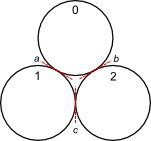
\includegraphics{figures/pyr2simple.png}
  \caption{A simple 2 layered pyramid.}
  \label{pyr2simple}
  % TODO: More figures? One with a downward arrow and the resulting impulses?
\end{figure}

Naturally, the more layers we add to our pyramids, the more complex these
interactions become, since we have to more contacts into account. For example,
in figure \ref{fig:pyr4-0}, to compute the impulse of the contact between discs
5 and 8, we have to take into accounts all the forces that act upon those two
discs. In particular, to compute the contact impulse between disc 5 and 8 we
have to take into account the contact impulses of all the disc-pairs $(2;5)$,
$(4;5)$, $(5;9)$, $(4;8)$, $(7;8)$, and $(8;9)$. Furthermore, we have to
translate the impulses in these adjacent contacts to the contact-space of the
contact between disc 5 and 8, in order to actually know what the contribution
is.

As can easily be imagined for this particular problem, the more layers we add,
the more contacts there are~\footnote{In fact, for a height $n$, we have
  exactly $\frac{3n}{2}(n-1)$ contacts: Each layer introduces $2n-2$ contacts
  between the new layer and the old, in addition to the $n-1$ contacts in the
  new layer. We can then prove the above by induction.}, and for each contact,
we have to take up to 10 other contacts into account when calculating its
impulse, as can easily be seen in figure \ref{fig:upto10}. Furthermore, as
contact impulses depend on adjacent contact impulses, we cannot easily
calculate an analytical solution. Instead, we have to compute the solution
numerically, by using intermediate estimates to iteratively produces better and
better estimates for the contact impulses until we reach convergence.

Because of the massive size of these problems, and the iterative nature of the
solver, computing the contact impulses in large pyramids is expensive on
traditional sequential architectures. We wish to explore the possibility and
efficiency of computing these contact dynamics by using the data parallel
architecture of GPUs.

\section{Goals}

We wish to calculate the contact impulses between discs in a 2-dimensional
system using Accelerate, a Haskell embedded language for expressing parallel
computations suitable for execution on a GPU. Since transferring data to and
from the GPU can incur significant overhead, and GPU programming in general
imposes constraints on how computations can be done, we also wish to run
performance tests, comparing the GPGPU implementation with implementations of
the solver running on traditional sequential hardware, in order to discuss the
efficiency of the implementation.

\section{Contact Dynamics}

We will focus on computing the impulses for a contact $\alpha$ of a body $i$ in
one timestep. For a body $i$, let $M_i$ be the $3 \times 3$ diagonal mass
matrix, with the third component of the diagonal being the inertia of $i$, let
$V_i$ and $V_i^-$ be the velocity vectors of the current and last timestep for
the body $i$, and let $R_i$ and $R_i^{ext}$ be the external and contact impulses
applied to the body. We then have the following relationship between motion
over time for the body $i$:

\begin{equation}
  M_i(V_i - V_i^-) = R_i + R_i^{ext}
\end{equation}

Clearly, if we can find the contact impulses for the body $i$, we can find the
velocity of the body in the current step.

In order to do this, we need to find the relative velocity for each contact
between $i$ and adjacent bodies. We call a contact $\alpha$, where each
$\alpha$ has two bodies in contact, called the candiate and the antagonist. The
relative velocity $v_\alpha$ is expressed from $V_{cd}$ and $V_{an}$ as
\begin{equation}
  v_\alpha =
  \begin{pmatrix}
    H_\alpha^{cd} &
    H_\alpha^{an}
  \end{pmatrix}
  \begin{pmatrix}
    V_{cd} \\
    V_{an}
  \end{pmatrix}
\end{equation},
where $H_\alpha^{cd}$ and $H_\alpha^{an}$ are rotational matrices for the angle
between the antagonist and candidate.

For the body $i$, we may then introduce the following equation
\begin{equation}
  v_i = H_i^TV_i
\end{equation}
where $v_i$ is the concatenated vector of relative velocities for the contacts
related to $i$ and $H_i$ is the concatenated vector of rotational matrices for a
specific body and it's contacts. By duality consideration, we may also show that
the following relationship between contact impulses $r_i$ and the resultant
impulse $R_i$ on body $i$ are
\begin{equation}
R_i = H_i r_i
\end{equation}

Letting $W_i = H_i^TM_i^{-1}H_i$, we now have
\begin{align}
  & M_i(V_i - V_i^-) = R_i + R_i^{ext} \\
  \Leftrightarrow \quad & H_i^T V_i - H_i^T V_i^-) = H_i^TM_i^{-1} R_i + H_i^T
  M_i^{-1} R_i^{ext}
  \\
  \Leftrightarrow \quad & v_i - v_i^{-} = H_i^T M_i^{-1}H_i r + H_i^T M_i^{-1} R^{ext} \\
  \Leftrightarrow \quad & v_i - v_i^{-} = W_i r + H_i^T M_i^{-1} R^{ext} \\
  \Leftrightarrow \quad & W_i r - v_i = -v_i^{-} - H_i^T M_i^{-1} R^{ext}
\end{align}
Where we call $-v_i^{-} - H_i^T M_i^{-1} R^{ext}$ our right-hand side (RHS).
Additionally, for a contact $\alpha$, we have the following relationship between
its impulse $r_\alpha$ and the relative velocity of the bodies in contact
$v_\alpha$:

\begin{equation}
  v_\alpha \geq 0, \quad r_\alpha \geq 0, \quad r_\alpha \cdot v_\alpha = 0
\end{equation}

Meaning that if two bodies are in contact, they are either moving away from
each other, relative to the contact normal, or they are pushing against each
other~\footnote{Additionally, there is the possibility that there is neither
  impulse nor velocity relative to the contact normal, but we can disregard
  this case, as it has no effect on the outcome}. This means, that if we can
find RHS, we can, by exclusion, find the impulse in a contact $\alpha$. For
finding the right-hand side, we use a series of continually improved estimates,
and this is where our Jacobi solver comes in.

\section{Initial Haskell implementation of the Jacobi solver}

The Jacobi method is an algorithm for determining the solution for a linear
system of equations. By regarding the contact impulses as our linear equations
(which makes sense since they rely on each other), the Jacobi method allows us
to iteratively refine a guess for the impulse values, until at some point they
converge.

The ordinary Haskell implementation uses the library \verb+hmatrix+, a ``purely
functional interface to basic linear algebra'', which internally uses GSL (the
GNU Scientific Library), as well as BLAS and LAPACK which are both low level
libraries for linear algebra. The entire code can be seen in appendix
\ref{app:seq}.

For each iteration of our Jacobi solver, we have to find the right-hand side of
\begin{equation}
  W_{\alpha\alpha} r_\alpha^{k+1} - v_\alpha^{k+1}= - H_i^T M_i^{-1} R_i^{ext}
  - \displaystyle\sum\limits_{\beta \neq \alpha} W_{\alpha\beta} r_\beta^k
\end{equation}
and solve the equation with regards to the constraints given above. To do this,
we use the function \verb+iter+, which takes a list of estimated impulses, a
list of all the contacts in the system, a list of external forces for each
contact, and precomputed lists of adjacent contacts and $W_{\alpha\alpha}$
values, and runs $k$ steps of the solver.

\begin{verbatim}
iter :: (Eq a, Num a) => a -> [Vector Double] -> [Contact] -> [Vector Double]
        -> [[Int]] -> [Matrix Double] -> [Vector Double]
iter 0 rs _ _ _ _ = rs
iter k rs cs ext adjs waas = iter (k-1) r_new cs ext adjs waas
    where
      rhss' = zipWith (sumWab cs rs) cs adjs
      rhss = zipWith (+) ext rhss'
      r_new' = zipWith solver rhss waas
      r_new = zipWith3 relaxer r_new' rs
                $ map ((1/) . fromIntegral . length) adjs
      relaxer new old relax = scale relax new + scale (1-relax) old
\end{verbatim}
Notice that we have added a relaxation term to each guess. It turned out to be
necessary in order to achieve convergence; without it, the total sum of
impulses would continue to grow forever.

The function \verb+iter+ relies on the function \verb+sumWab+ which takes a
contact and sums up the products of adjacent contacts and their impulses.
\begin{verbatim}
sumWab :: [Contact] -> [Vector Double] -> Contact -> [Int] -> Vector Double
sumWab cs rs c adjs =
    neg $ foldr add (fromList [0, 0]) prods
        where
          prods = zipWith mXv wabs $ pick rs adjs
          wabs = map (wab c) $ pick cs adjs
\end{verbatim}

\section{Parallel implementation in Accelerate}

\section{Results}

\section{Conclusion}

\end{document}
